\chapter{Valutazione sperimentale}\label{chap:experiments}


\noindent Questo capitolo descrive la valutazione sperimentale. Vi sono esposti il protocollo con
cui le ipotesi formulate nel capitolo precedente sono tradotte in confronti controllati e la
metodologia statistica adottata per sintetizzarli; l'infrastruttura materiale su cui le campagne
si fondano; i dataset, la griglia delle configurazioni e le metriche con cui i risultati sono
misurati; il termine di paragone banale che dà una scala ai valori assoluti; gli esperimenti
condotti, con il collegamento esplicito alle ipotesi che essi verificano; e lo studio di ablazione
che isola il contributo dei singoli componenti della strategia principale. L'effetto della
potatura sul tempo di esecuzione, che non è una proprietà delle configurazioni ma un esito, è
discusso insieme ai risultati.

% =======================================================================================
\section{Protocollo di verifica}\label{sec:verification}

Il protocollo di verifica si fonda su cinque scelte, adottate per evitare errori di
interpretazione che si erano effettivamente presentati nel corso del lavoro.

\paragraph{Confronto appaiato.} Ogni configurazione potata è confrontata con la medesima
configurazione non potata, sullo stesso dataset, la stessa esecuzione e la stessa soglia. Il
confronto fra medie aggregate su configurazioni diverse è stato evitato perché sensibile alla
composizione del campione.

\paragraph{Unità di analisi dichiarata.} L'unità di analisi è la \emph{configurazione}, cioè la
tripletta dataset, soglia e ripetizione, e non la cella nulla. La scelta è motivata dalla
struttura del sistema: le imputazioni di una stessa esecuzione non sono indipendenti, perché
condividono l'ordine delle regole e i cluster, e trattarle come osservazioni separate
moltiplicherebbe artificialmente la numerosità campionaria. Ne segue che la numerosità dei test è
quella delle configurazioni --- decine, non migliaia --- e che la potenza statistica è
conseguentemente limitata.

\paragraph{Controllo della vacuità.} Il confronto è privo di contenuto in due circostanze
distinte. La prima è che il file di regole prodotto dalla potatura sia identico a quello di
partenza: la potatura non ha fatto nulla e non vi è nulla da misurare. La seconda, meno evidente,
è che la configurazione di partenza non produca \emph{alcuna} imputazione: la potatura non è
vacua, ma il confronto lo è, perché tutte le grandezze di qualità valgono zero in entrambi i
bracci. Il sistema di valutazione segnala entrambe le circostanze, e le configurazioni
corrispondenti sono escluse dai test e contate a parte: trattarle come esiti nulli introdurrebbe
una massa di zeri artificiale, e le tratterebbe come evidenza di assenza di effetto.

\paragraph{Controllo casuale.} Per attribuire un effetto a un ordinamento --- e non al mero atto
di riordinare --- è necessario un termine di paragone casuale. Sono state impiegate permutazioni
con seme fissato, in numero di tre e indipendenti fra loro; il confronto è condotto sia contro
ciascuna permutazione, sia contro la loro media per configurazione.

\paragraph{Verifica indipendente delle condizioni.} Le condizioni teoriche sono verificate su
stati reali del dataset, non soltanto per implicazione logica: per ogni regola rimossa dalla
condizione \Vtwo{} si controlla che una regola coprente sopravvissuta eserciti effettivamente il
veto sugli stessi testimoni.

% =======================================================================================
\section{Metodologia statistica}\label{sec:statistics}

Il confronto fra configurazione potata e configurazione di partenza è un confronto appaiato su
variabili che non si distribuiscono in modo normale --- il numero di imputazioni corrette è una
conta con molti valori estremi e molte differenze nulle --- e il test adottato è quindi il test
dei ranghi con segno di Wilcoxon \cite{wilcoxon1945individual}.

\paragraph{Il test.} Per ogni confronto si considerano le differenze $\Delta_i = B_i - A_i$ fra la
variante e la configurazione di partenza sulla medesima configurazione, si scartano le differenze
nulle e si ordinano i valori assoluti. La statistica è la somma dei ranghi delle differenze
positive, $W^+$. Quando non vi sono ranghi medi e il numero di differenze non nulle non supera
venticinque, la distribuzione nulla è calcolata in forma \emph{esatta} per enumerazione; negli
altri casi si impiega l'approssimazione normale con correzione di continuità e correzione per i
ranghi medi. Il test è a due code. Il numero di differenze non nulle, e non il numero di
configurazioni, è la numerosità effettiva del test: le colonne $n$ e $n_{\text{test}}$ della
\autoref{tab:statistics} li riportano entrambi.

\paragraph{Dimensione dell'effetto.} La significatività non dice quanto grande sia l'effetto, e con
numerosità dell'ordine di alcune decine è possibile ottenere valori di $p$ piccoli per differenze
di una sola unità. Si riporta quindi la \emph{differenza mediana} --- robusta rispetto agli
estremi --- e la correlazione rank-biserial per campioni appaiati,
$r = (W^+ - W^-) / (W^+ + W^-)$, che è l'analogo non parametrico della $d$ di Cohen: valori
assoluti intorno a $0.1$, $0.3$ e $0.5$ indicano effetto piccolo, medio e grande.

\paragraph{Intervalli di confidenza.} Per la differenza mediana si riporta un intervallo di
confidenza al \SI{95}{\percent} ottenuto per ricampionamento delle coppie con reimmissione
(diecidimila replicazioni, seme fissato), con il metodo dei percentili. L'intervallo è ampio per
costruzione, data la numerosità, ed è riportato per rendere esplicita l'incertezza invece di
affidare la lettura alla sola soglia di significatività.

\paragraph{Confronti multipli.} Il lavoro verifica sette ipotesi primarie su più metriche e
decine di configurazioni, e la probabilità di almeno un falso positivo cresce con il numero di
test. I test che costituiscono la famiglia primaria --- quelli su cui poggiano le conclusioni del
\autoref{chap:results} --- sono cinque, dichiarati in
\texttt{pruning/stats\_effects.py}, e per essi si riporta il valore di $p$ corretto con la
procedura di Holm \cite{holm1979simple}, che controlla la probabilità di almeno un rifiuto errato
sull'intera famiglia. La correzione è conservativa e va letta come tale: il suo effetto è di
alzare la soglia, non di abbassarla.

\begin{table}[htbp]
\centering
\caption{Test della famiglia primaria. $\Delta$ è la differenza fra variante e configurazione di
partenza, $r$ la correlazione rank-biserial, l'intervallo è quello di confidenza al
\SI{95}{\percent} della differenza mediana. $p$ è il valore grezzo, $p_{\text{Holm}}$ quello
corretto per i cinque test della famiglia.}
\label{tab:statistics}
\scriptsize
\begin{tabular}{@{}lrrrll@{}}
\toprule
confronto & $n$ & $n_{\text{test}}$ & mediana $\Delta$ [IC \SI{95}{\percent}] & $r$ & $p$ \;/\; $p_{\text{Holm}}$ \\
\midrule
\str{A5b} su Bridges, corrette      & 50 & 39 & $+0.5$ $[0.0,\ +2.0]$ & $+0.510$ & $0.0053$ / $0.0159$ \\
\str{A5b} su Bridges, errori        & 50 & 35 & $-1.0$ $[-2.0,\ 0.0]$ & $-0.905$ & $2.5\cdot10^{-6}$ / $1.3\cdot10^{-5}$ \\
taratura conservativa, corrette     & 10 & 0  & $0.0$ $[0.0,\ 0.0]$ & $0.000$ & $1.0000$ / $1.0000$ \\
ordinamento, primo contro originale & 15 & 13 & $+2.0$ $[+1.0,\ +5.0]$ & $+1.000$ & $0.0016$ / $0.0064$ \\
ordinamento, primo contro casuale   & 15 & 8  & $0.0$ $[0.0,\ +0.7]$ & $+0.083$ & $0.8878$ / $1.0000$ \\
\bottomrule
\end{tabular}
\end{table}

\begin{figure}[htbp]
\centering
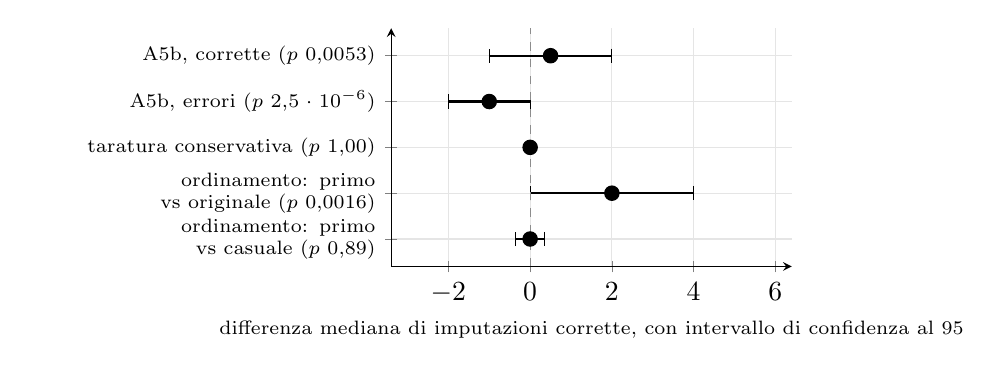
\begin{tikzpicture}
\begin{axis}[
    width=0.55\textwidth,
    height=0.38\textwidth,
    xmin=-3.4, xmax=6.4,
    ymin=0.4, ymax=5.6,
    ytick={1,2,3,4,5},
    yticklabels={{ordinamento: primo vs casuale ($p$ 0,89)},
                 {ordinamento: primo vs originale ($p$ 0,0016)},
                 {taratura conservativa ($p$ 1,00)},
                 {A5b, errori ($p$ $2{,}5\!\cdot\!10^{-6}$)},
                 {A5b, corrette ($p$ 0,0053)}},
    yticklabel style={font=\scriptsize, align=right, text width=4.3cm},
    xlabel={differenza mediana di imputazioni corrette, con intervallo di confidenza al \SI{95}{\percent}},
    xlabel style={font=\scriptsize},
    grid=major,
    grid style={black!10},
    axis y line=left,
    axis x line=bottom,
    clip=false,
]
\addplot[only marks, mark=*, mark size=2.6pt,
         error bars/.cd, x dir=both, x explicit, error bar style={thick}]
    coordinates {
        (0.0,1) +- (0.35,0)
        (2.0,2) +- (2.0,0)
        (0.0,3) +- (0.0,0)
        (-1.0,4) +- (1.0,0)
        (0.5,5) +- (1.5,0)
    };
\draw[dashed, black!45] (axis cs:0,0.4) -- (axis cs:0,5.6);
\end{axis}
\end{tikzpicture}
\caption{Test della famiglia primaria: differenza mediana di imputazioni corrette e intervallo di
confidenza al \SI{95}{\percent} ottenuto per ricampionamento. I valori di $p$ sono quelli grezzi;
quelli corretti con la procedura di Holm sono nella \autoref{tab:statistics}. La linea verticale
indica l'assenza di differenza.}
\label{fig:forest}
\end{figure}

La \autoref{tab:statistics} si legge in due modi. Sul piano della significatività, i due test
sulla potatura aggressiva e quello sull'ordinamento sopravvivono alla correzione per confronti
multipli; il confronto fra riordino informato e riordino casuale non è significativo, ed è il
risultato che falsifica l'ipotesi H14, non un test fallito. Sul piano della dimensione
dell'effetto, i due test che sopravvivono hanno valori di $r$ medio e grande, mentre gli altri
hanno effetti trascurabili o nulli: la distinzione conta perché una differenza mediana di mezza
imputazione, pur significativa su cinquanta configurazioni, non è un guadagno utilizzabile, ed è
la ragione per cui il \autoref{chap:results} riporta le somme delle differenze e non soltanto i
valori di $p$.

Due limiti della metodologia statistica vanno dichiarati. Il primo è che la famiglia primaria è
stata dichiarata \emph{dopo} la raccolta dei dati, sebbene prima del calcolo dei test: non vi è
quindi pre-registrazione, e la correzione di Holm protegge dalla molteplicità ma non dalla
selezione dei confronti. Il secondo è la potenza: con alcune decine di configurazioni, differenze
piccole rispetto alla variabilità fra dataset non sono distinguibili dal caso, e l'assenza di
significatività non va letta come assenza di effetto.

\section{Setup sperimentale}\label{sec:setup}

\paragraph{Infrastruttura.} La valutazione si fonda su due strumenti sviluppati per il lavoro: un
\emph{pruner} esterno, che riscrive il file delle regole secondo la strategia richiesta, e un
\emph{benchmark} che esegue il sistema nella configurazione di partenza e in quella potata,
raccoglie le metriche e le confronta. Il sistema oggetto di studio non è mai stato modificato
durante la valutazione esterna: l'eseguibile impiegato è quello originale, verificato per
checksum all'inizio e alla fine delle campagne.

\paragraph{Isolamento delle esecuzioni.} Ogni esecuzione avviene in una cartella di lavoro
dedicata, che viene ripulita prima dell'esecuzione successiva. Le esecuzioni sono condotte in
sequenza, mai in parallelo: la cartella di lavoro è condivisa e due esecuzioni simultanee
sovrascriverebbero reciprocamente gli output. La circostanza è stata verificata sperimentalmente
e ha richiesto di rieseguire alcune configurazioni.

\paragraph{Riproducibilità.}\label{sec:reproducibility}
Tutti i numeri presentati nel \autoref{chap:results} sono ricalcolabili dai file di risultati
prodotti dalle campagne, e la ricalcolabilità è verificata automaticamente: una procedura di
verifica ricalcola i valori asseriti nella documentazione e li confronta con quelli memorizzati,
segnalando ogni divergenza. La procedura copre \num{67} asserzioni numeriche, incluse quelle
relative alle condizioni teoriche. I dettagli sono nell'\autoref{app:reproducibility}.

% =======================================================================================
\section{Dataset e configurazioni}\label{sec:datasets-exp}

La valutazione impiega tre famiglie di dataset, scelte fra quelle disponibili nell'archivio
secondo criteri di utilizzabilità e di diversità strutturale
(\autoref{tab:families}). La \autoref{tab:grid} riassume la griglia effettivamente coperta.

\begin{table}[htbp]
\centering
\caption{Griglia sperimentale. ``Configurazioni'' è il numero di triplette
\emph{dataset, run, soglia} distinte.}
\label{tab:grid}
\footnotesize
\begin{tabular}{lrrrr}
\toprule
famiglia & dataset & run & soglie & configurazioni \\
\midrule
Bridges    & 5 & 1--5 & 3, 9, 15 & 60 \\
Glass      & 5 & 1--5 & 3, 9, 15 & 75 \\
Restaurant & 4 & 1--3 & 3, 6     & 22 \\
\midrule
totale     & 14 & & & \textbf{157} \\
\bottomrule
\end{tabular}
\end{table}

Le tre famiglie differiscono per caratteristiche che si riveleranno determinanti
nell'interpretazione dei risultati: il numero di regole disponibili, la distribuzione delle celle
nulle fra tuple con una sola cella nulla e tuple con più celle nulle
(\autoref{sec:two-branches}), e la quota di imputazioni che il sistema ottiene per via esatta
(\autoref{sec:mechanism}).

Due famiglie dell'archivio non sono state impiegate per l'intera griglia. La famiglia Nursery
comprende cinque file di regole --- le soglie \num{3}, \num{6}, \num{9}, \num{12} e \num{15}
--- ma nessun dataset e nessun file di tuple iniziali, quindi nessuna configurazione eseguibile:
è il residuo di una fase di estrazione di cui non è stato distribuito il dato. La famiglia
Physician comprende venticinque configurazioni piene di \num{103592} righe, di dimensioni tali da
rendere impraticabile una campagna, e quattro versioni remodulate il cui materiale di ground truth
presenta indici di riga eccedenti il dataset (\autoref{chap:defects}). Le versioni remodulate sono
state rese eseguibili escludendo le celle non localizzabili, ed è su di esse che si fonda la prova
sulla quarta famiglia i cui esiti sono riportati nella \autoref{sec:physician}.

% =======================================================================================
\section{Metriche}\label{sec:metrics}

Le metriche adottate sono le seguenti. Sia $C$ l'insieme delle celle per cui è disponibile il
valore di ground truth; si ricordi che tale insieme non coincide necessariamente con l'insieme
delle celle nulle del dataset (\autoref{sec:datasets}).

\begin{table}[htbp]
\centering
\caption{Metriche adottate. $C$ è l'insieme delle celle con valore di ground truth disponibile,
$I \subseteq C$ l'insieme delle celle imputate, $K \subseteq I$ quelle imputate correttamente.}
\label{tab:metrics}
\footnotesize
\begin{tabular}{@{}llp{4.4cm}@{}}
\toprule
metrica & definizione & che cosa falsifica \\
\midrule
copertura & $|I| / |C|$ & una potatura che, togliendo regole, fa rifiutare al sistema celle che
prima valorizzava \\
precisione & $|K| / |I|$ & una potatura che rende accettate imputazioni di qualità peggiore \\
accuratezza & $|K| / |C|$ & l'effetto complessivo; è il prodotto delle due precedenti \\
errori & $|I| - |K|$ & l'aumento del danno, che l'accuratezza può mascherare quando la copertura
cresce \\
quota esatta & frazione di $I$ ottenuta per via esatta & la composizione delle imputazioni, primo
fattore del meccanismo (\autoref{sec:mechanism}) \\
preprocessing & secondi per riscrivere il file delle regole & il costo dell'analisi, da
confrontare con il risparmio in esecuzione \\
esecuzione & secondi del sistema, a parità di configurazione & l'effetto sul costo, che
non segue la riduzione (\autoref{sec:res-cost}) \\
\bottomrule
\end{tabular}
\end{table}

La distinzione fra copertura e precisione è essenziale nel seguito. Un metodo basato su vincoli
può rifiutare di imputare, e una potatura che rimuova regole può indurre nuovi rifiuti: in quel
caso la copertura cala mentre la precisione può salire, e l'accuratezza può restare invariata. La
lettura congiunta delle due metriche è quindi necessaria, e le analisi che seguono la rispettano
sistematicamente.

Per i dataset a prevalenza testuale (Restaurant) il confronto esatto fra stringhe è troppo
severo: due ragioni sociali che differiscono soltanto per la forma societaria finale sono contate
come valori diversi pur designando la stessa entità. Per questa famiglia si adotta pertanto una
soglia di similarità normalizzata di Levenshtein pari a \num{0.8}, e le metriche testuali sono
riportate separatamente da quelle esatte.

% =======================================================================================
% =======================================================================================
\section{Termine di paragone banale}\label{sec:trivial-baseline}

Le metriche del capitolo sono differenze rispetto alla medesima configurazione non potata: dicono
se la potatura migliora o peggiora il risultato del sistema, non se il risultato del sistema sia
buono in assoluto. Per dare una scala, la \autoref{tab:trivial} confronta l'accuratezza del
sistema con quella di un imputatore banale che sostituisce a ogni cella la \emph{moda} della
colonna, calcolata sui valori osservati. La moda è un termine di paragone volutamente povero ---
non impiega alcuna dipendenza --- ed è calcolata sulle stesse celle valutate dal sistema.

\begin{table}[htbp]
\centering
\caption{Confronto con un imputatore banale (moda di colonna) sulle stesse celle valutate. La
copertura della moda è totale per costruzione. I valori si riferiscono alle configurazioni con
schema allineato: \num{6} configurazioni di Bridges (prima ripetizione, soglie 3 e 9) e le
\num{2} versioni eseguibili di Physician.}
\label{tab:trivial}
\footnotesize
\begin{tabular}{@{}lrrrrr@{}}
\toprule
famiglia & configurazioni & celle & accuratezza moda & accuratezza sistema & copertura sistema \\
\midrule
Bridges   & \num{6} & \num{224} & \num{0.536} & \num{0.545} & \SI{61.6}{\percent} \\
Physician & \num{2} & \num{40}  & \num{0.275} & \num{0.150} & \SI{35.0}{\percent} \\
\bottomrule
\end{tabular}
\end{table}

La lettura del confronto è duplice, e va data per intero. Su Bridges la moda raggiunge
un'accuratezza praticamente uguale a quella del sistema (\num{0.536} contro \num{0.545}) con
copertura totale: su questo dataset la qualità \emph{assoluta} delle imputazioni non è il punto di
forza del sistema, e il valore che il lavoro misura è quello che la potatura aggiunge o toglie a
parità di sistema. Su Physician il divario è più netto e in direzione opposta: la moda è migliore
del sistema (\num{0.275} contro \num{0.150}), perché il sistema copre il \SI{35}{\percent} delle
celle e, fra quelle che copre, non sempre indovina.

Due avvertenze delimitano la portata del confronto. La prima è che il perimetro della tesi non
comprende il confronto con metodi di imputazione alternativi (\autoref{sec:res-limits}): la moda
non è un concorrente del sistema ma una \emph{scala} per i suoi numeri. La seconda è che
l'accuratezza è misurata soltanto sulle celle introdotte artificialmente, quelle per cui esiste il
ground truth: il sistema può imputare anche celle nulle preesistenti, che non entrano in questa
misura (\autoref{sec:datasets}).

\section{Esperimenti condotti}\label{sec:experiments}

Le campagne condotte ammontano complessivamente a \num{1618} esecuzioni del sistema in
configurazione potata, oltre alle esecuzioni di riferimento. Esse non sono un insieme di prove
giustapposte: ciascuna risponde a una delle ipotesi enunciate nel \autoref{chap:hypotheses}, e la
\autoref{tab:experiments} esplicita il collegamento, perché è su di esso che poggia la lettura
degli esiti.

\begin{table}[htbp]
\centering
\caption{Esperimenti condotti, obiettivo e ipotesi verificate. La colonna ``bracci'' indica che
cosa viene confrontato; la colonna ``risultati'' la sezione in cui l'esito è riportato.}
\label{tab:experiments}
\footnotesize
\begin{tabular}{@{}clp{4.4cm}ll@{}}
\toprule
\# & obiettivo & bracci confrontati & ipotesi & risultati \\
\midrule
E1 & equivalenza della potatura garantita & \str{veto-cover} contro configurazione di partenza, su tre famiglie & H6 & \ref{sec:res-vetocover} \\
E2 & verifica indipendente della copertura & ricostruzione dei testimoni del veto per ogni regola rimossa & H7 & \ref{sec:res-vetocover} \\
E3 & effetto della potatura aggressiva & \str{A5b} contro configurazione di partenza, su tre famiglie e tre soglie & H8, H11 & \ref{sec:res-a5b}, \ref{sec:res-boundary} \\
E4 & attribuzione del guadagno & riordino per precisione, riordino inverso, tre permutazioni casuali & H14 & \ref{sec:negative-results} \\
E5 & ablazione dei componenti & ciascun componente di \str{A5b} da solo, la combinazione, la somma & H8 & \ref{sec:ablation} \\
E6 & proporzionalità fra riduzione e tempo & tempi di esecuzione appaiati, per strategia e configurazione & H16 & \ref{sec:res-cost} \\
E7 & strategie esatte alternative & \str{score-argmin} con tre politiche sui veti, su Bridges e Glass & H1, H2 & \ref{sec:score-argmin} \\
\bottomrule
\end{tabular}
\end{table}

Due precisazioni completano il disegno. La prima riguarda le configurazioni \emph{vacue}: le
combinazioni in cui la strategia non rimuove alcuna regola producono un file identico a quello di
partenza, e sono escluse dai test e conteggiate a parte. La seconda riguarda l'ordine di
esecuzione: le campagne sono state condotte in modo strettamente sequenziale, perché la cartella
di lavoro del sistema è condivisa fra esecuzioni e due esecuzioni simultanee sovrascrivono
reciprocamente gli output senza segnalare alcun errore. La circostanza è stata verificata
sperimentalmente, ed è la ragione per cui non si riportano misure di tempi concorrenti.

\section{Studio di ablazione}\label{sec:ablation}

La strategia \str{A5b} è una combinazione di due interventi: un riordino delle regole a soglia di
destra nulla e una potatura adattiva. Per stabilire quale dei due produca il guadagno, entrambi
sono stati misurati anche separatamente, sulle stesse configurazioni.

\begin{table}[htbp]
\centering
\caption{Ablazione di \str{A5b} su Bridges, configurazioni comuni. Le variazioni sono rispetto
alla medesima configurazione non potata.}
\label{tab:ablation}
\footnotesize
\begin{tabular}{lrrrr}
\toprule
componente & riduzione RFD & $\Delta$ corrette & $\Delta$ errori & esito \\
\midrule
\str{exact-priority} (solo)     & \SI{0}{\percent}   & $+25$ & $-53$ & non stabile fra soglie \\
\str{dom-sub-adaptive} (solo)   & \SI{81}{\percent}--\SI{87}{\percent} & $-20$ & $+20$ & danneggia \\
\textbf{\str{A5b} (combinazione)} & \SI{81}{\percent}--\SI{87}{\percent} & $\mathbf{+45}$ & $\mathbf{-32}$ & \textbf{migliora} \\
\midrule
somma dei due componenti & & $+5$ & & \\
\textbf{sinergia} & & $\mathbf{+40}$ & & \\
\bottomrule
\end{tabular}
\end{table}

Il risultato dell'ablazione è che \emph{nessuno dei due componenti funziona da solo}: il riordino
migliora il risultato a una soglia e lo peggiora all'altra, mentre la potatura adattiva lo
peggiora sistematicamente. La combinazione è invece stabile e positiva. La differenza fra il
guadagno osservato ($+45$) e la somma dei due componenti isolati ($+5$) è pari a $+40$, e
costituisce una \emph{sinergia} che va spiegata, non registrata.

La spiegazione è che i due interventi agiscono su fattori diversi del medesimo prodotto. La
potatura adattiva modifica la \emph{composizione} dei candidati --- quali regole concorrono a
determinare il valore --- e quindi la quota di imputazioni ottenute per via esatta; il riordino
modifica la \emph{sequenza} con cui i cluster vengono tentati e, nella procedura a più celle nulle,
determina quale cluster scrive per ultimo, quindi quante celle vengono effettivamente valorizzate.
Presi singolarmente, il primo peggiora la qualità delle imputazioni senza aumentarne il numero, il
secondo aumenta il numero di imputazioni senza migliorarne la composizione; applicati insieme,
producono un aumento di entrambi i fattori, e il guadagno risultante supera la somma dei guadagni
isolati. Il \autoref{sec:mechanism} verifica questa lettura sui tre regimi osservati --- Bridges,
Glass e Restaurant --- e ne ricava il criterio diagnostico.

Va sottolineato un limite del disegno di ablazione: le configurazioni comuni ai tre bracci sono
venti, e la lettura della sinergia poggia quindi su un campione più piccolo di quello della
campagna principale. L'ablazione identifica il meccanismo, non ne stabilisce la generalità.

% =======================================================================================
